	
	%opening
	\title{Can computers think?}
	\author{M. Girish}
	\documentclass[a4paper]{article}
	\usepackage[none]{hyphenat}
	\usepackage{graphicx}
	\usepackage{wrapfig}
	\begin{document}
	
	\maketitle
	
	\begin{abstract}
	Thinking is a non-trivial process. In its true essence thinking is what a \textit{being} is capable of. A sophisticated process which involves past knowledge
	and \textit{free will}. Experiments involving thoughtful actions can be used to differentiate a machine from human. Computers cannot spawn a \textit{thought-process} like humans.
	\paragraph{Keywords} \textit{artificial intelligence, consciousness, free will, intentionality, thought-process}
	\end{abstract}
	
	\section{Any form of computation is mechanical and doesn't need thinking}
	\paragraph{}
	\textit{If computers can think, then what qualities would they express or possess?}
	\paragraph{}They would converge to a decision based on experiences and presuppositions. There would be a bias
	in its choices for rationality may not always be an outcome.
	\paragraph{}
	\textit{What is thinking, where does it originate, and how does it perpetuate?}
	\paragraph{}
	Thought as a random occurrence in our mind would have a more simpler circuitry for computers. Can they
	rewire their thoughts by manipulating the programs to decide and make choices through their own \textit{free will}? This process may not have a finite number of steps. This discussion leads to self awareness and most importantly \textit{consciousness}. Consciousness in simpler terms means self awareness. The computers becoming self aware of its existence cannot happen unless programmed to do so. To program this, a programmer would have to define cases as to what constitutes consciousness and specify when can computers arrive at a result to indicate that it is conscious. This may not be an exhaustive list and hence a futile attempt in making computers \textit{aware}.
	\paragraph{}
	\textit{What is consciousness and how are thoughts related to it?}
	\paragraph{}
	When we say that a computer can think and take actions, we say that it does with minimal programming or human
	intervention. It can sense the surroundings through its sensors, interpret the physical quantities and formulate
	actions based on experience.
	\paragraph{}
	\textit{What makes a computer thoughtful?}
	\paragraph{}
	An example that could be thought here is of a lawn mower. It cuts down grass to keep a garden tidy. So, a 
	lawn mower operated by a gardener would just cut down whatever it can get in its way - insects, grass, weed, flowers,
	anything and everything. The onus is on the gardener to control its movement and how much time it spends at a particular
	location. A further advancement to this machine is - whether it can operate in a certain area of action without gardener's
	involvement. The gardener's task is only to fix the boundaries for the mower to operate.
	The mower is now capable of measuring distance from its starting point and gauge the area of operation. Also, the gardener may
	fix operational hours and just let it be. This mower now operates under certain program but still cannot make decisions on which
	grass to cut, whether to skip any earthworms and mow parts depending on a optimal path. The mower with an autonomous computer
	that could think, would have to think like a gardener. The gardener senses environment around him and ventures mowing based on external
	factors such as weather and soil conditions. The machine would have to rewire and register memories of new events and pictures of the
	vegetation around it. It needs to think and compute surroundings; to not get in contact with any insect or human. What happens when unknown
	conditions in environment affects the machine? Would it know when to stop and restart? Can it make a decision on its own? Can machine
	understand and allocate for its own survival and longevity? Can a machine consider itself as a living being and take action to 
	nurture itself and avoid conflict with nature for its survival? The neural network of a machine and its dynamic wiring to make a choice
	or action depends on this process of thinking known as a \textit{thought-process}. It is the key to any problem solving - by using one's
	experience to pave way for newer solutions. Only by past solution to similar problems can humans tend to innovate on solving existing ones.
	Moreover, after finding a solution how can machine evaluate and reassess for its correctness without a verification model designed autonomously?
	\section{Turing test and its effectiveness}
	\paragraph{}
	\textit{Is the Turing test\cite{turing50} meaningful and valid?}
	\paragraph{}
	Turing suggested that if a computer and a human being were hidden behind a screen, and another
	human being were given the task of interrogating each of them, it would be reasonable to conclude that the computer was conscious if the interrogator could not distinguish it
	from the human being (Figure 1). There have been many variations of the Turing test proposed, some by Turing himself, and there are annual contests based on Turing test. Thus far, no computer has
	passed the Turing test (by general consensus), although some have come close. Several plausible characteristics have been proposed — free will, restricted access (only the thinker experiences his thoughts), incorrigibility (only the thinker knows with certainty the content of his thought), qualia (raw sensory experience), etc.
		\begin{figure}
			\centering
			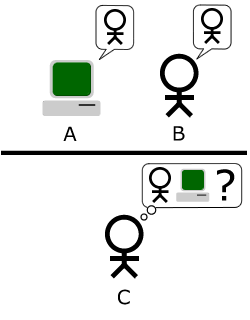
\includegraphics[height=5cm]{Turing_Test}
				\caption{The ``standard interpretation" of the Turing Test, in which player C, the interrogator, is given the task of trying to determine which player - A or B - is a computer and which is a human. The interrogator is limited to using the responses to written questions to make the determination. Image adapted from Saygin, 2000\cite{saygin00}}
		\end{figure}
		
	\section{Intentionality behind computation}
	\paragraph{}
	The classic argument that computation inherently lacks intentionality (meaning) can be inferred from Searle's Chinese Room analogy \cite{searle80}. Intentionality is a primary characteristic of human mind. The actions are driven by it and thoughts are the fuel. In case of a computer, it manifests the intentionality of its programmer. The programmer could be another program recursively. Yet, the base program would be the one of a human programmer. So it derives the intentionality from a human in principle. Searle concludes through his analogy that computation has no intrinsic intentionality, but only secondary intentionality imparted by programmers. Computation is not \textit{thinking}, but a mechanical process. 
	\begin{thebibliography}{9}
		
		\bibitem{turing50}
		 A.M Turing,
		\textit{Computing Machinery and Intelligence, Mind},
		Volume LIX, Issue 236, October 1950, Pages 433–460
		
		\bibitem{egnor11}
		Michael Egnor,
		\textit{Can a Computer Think?},
		Evolution News, March 2011
		
		\bibitem{searle80}
		Searle, John. R.
		\textit{Minds, brains, and programs. Behavioral and Brain Sciences},
		3 (3): 417-457
		
		\bibitem{saygin00}
		Saygin, A.P.; Cicekli, I.; Akman, V.
		\textit{Turing Test: 50 Years Later, Minds and Machines},
		10 (4): 463-518
		
	\end{thebibliography}
	\end{document}
